% Shared approved exhibit definitions for both CTJ layouts.
% Author: Andrew Walther. Updated: 2026-10-27.
% Figure sources: code/20_manuscript_figure_revision.R; no simulation rerun.
% Table 1 example maps: code/25_design_assignment_figures.R (illustrative surface).
% Starred floats span both reading columns; every macro is called once per build.

% One example map per Table 1 row, vertically centered with padding between rows;
% \CTJCat sets each design's category on an italic line under its name.
\newcommand{\CTJCat}[1]{\newline{\footnotesize\textit{#1}}}
\newcommand{\CTJThumb}[1]{\raisebox{-0.5\height}{\includegraphics[width=1.9cm]{../figures/compact/design_thumbs/thumb_#1.pdf}}\rule[-1.05cm]{0pt}{2.2cm}}
\newcommand{\CTJDesignTable}{%
\begin{table*}[!htb]
\small
\centering
\caption{Treatment assignment designs on the 100-cluster grid and their North Carolina (NC) adaptations, each with its category (italic) and one example assignment on the grid (blue, treated; white, control). Every example uses the incidence surface in the first row, a representative spatial surface (incidence dependence $\rho_X=0.5$) drawn for illustration. Numbers in the Balanced Quartiles example give each cluster's incidence quartile; percentages in the Incidence-Guided Saturation example give each quadrant's treated share. Incidence is the simulated grid covariate or the observed annual cluster rate. Two related variants, Saturation Quadrants (randomly ordered quadrants) and Balanced Halves (balancing within incidence halves), performed similarly to their retained counterparts and are reported in the supplementary information (SI).}
\label{tab:allocation-rules}
\begin{tabular}{>{\raggedright\arraybackslash}m{0.16\linewidth}c>{\raggedright\arraybackslash}m{0.35\linewidth}>{\raggedright\arraybackslash}m{0.27\linewidth}}
\toprule
Design & Example (grid) & Grid (100 clusters) & NC (58 clusters) \\
\midrule
\textit{Incidence surface} & \CTJThumb{incidence} & Representative incidence surface used in the design examples below; darker cells represent higher incidence, and dashed lines mark quadrant boundaries. & Observed annual SUD rate of each cluster. \\
Checkerboard\CTJCat{Fixed spatial interspersion} & \CTJThumb{1} & Treat alternating clusters in a checkerboard pattern, so no two clusters that share an edge are in the same arm (50 treated). & Deterministic map version that visits clusters from most to fewest neighbors and gives each the arm less common among its assigned neighbors (27 treated). \\
High Incidence Focus\CTJCat{Incidence targeting} & \CTJThumb{2} & Treat the 50 clusters with the highest incidence, with ties broken at random (50 treated). & Treat the clusters with the highest observed rate (29 treated). \\
Isolation Buffer\CTJCat{Spatial separation} & \CTJThumb{4} & Treat clusters one at a time, each chosen at random from the untreated clusters with no treated neighbor, until none remain, so no two treated clusters are neighbors (about 21 treated with queen neighbors). & Same rule on the NC adjacency graph (about 16 treated). \\
$2\times2$ Blocking\CTJCat{Local spatial balance} & \CTJThumb{5} & Divide the grid into 25 blocks of $2\times2$ clusters and treat two randomly chosen clusters in each block (50 treated). & Spatial blocking, which treats a random half (rounded) of each of 14 groups formed each year by $k$-means clustering on location, incidence rank and log-population (27--31 treated by year). \\
Balanced Quartiles\CTJCat{Incidence balance} & \CTJThumb{6} & Divide clusters into quartiles of incidence rank and randomly treat half of the clusters in each quartile (50 treated). & Same rule with observed rates (29 treated). \\
Incidence-Guided Saturation\CTJCat{Incidence-ordered regional saturation} & \CTJThumb{8} & Treat a random 80\%, 60\%, 40\% and 20\% of the clusters in the four $5\times5$ quadrants, ordered from highest to lowest mean incidence (50 treated). & Same rule with four fixed geographic regions, ordered by the mean rank of their clusters' observed rates (29 treated). \\
Simple Random Sampling\CTJCat{Unrestricted reference} & \CTJThumb{9} & Treat a completely random half of the clusters (50 treated). & Same rule (29 treated). \\
\bottomrule
\end{tabular}
\end{table*}
}

\newcommand{\CTJGridTable}{%
\begin{table*}[!htb]
\small
\centering
\caption{Grid benchmark at $\tau=1$ with queen contiguity. Each regime-specific entry averages 80 scenarios (five incidence configurations, four outcome-dependence values $\rho$ and four spillover-magnitude values $\gamma$). MSE is the mean squared error of the estimate of $\tau$, and coverage is the proportion of 95\% $t$-based confidence intervals (CIs), with a degrees-of-freedom-corrected standard error, that contain $\tau$. Both use the spatial lag model that includes the true spillover term. The ratio to SRS divides each design's MSE by that of simple random sampling (SRS), which randomly selects 50 of the 100 clusters for treatment. Its 95\% interval is one plus the paired design-minus-SRS interval for the mean difference in MSE across the 50 independent configuration-by-surface units, divided by the SRS MSE, so an interval excluding 1 indicates a difference larger than simulation error (no adjustment for multiple comparisons).}
\label{tab:grid-srs}
% SOURCE: results/srs_benchmark/manuscript_regime_means.csv (MSE, coverage);
% results/srs_benchmark/manuscript_paired_ratios.csv (ratios; code/19 from code/15).
\setlength{\tabcolsep}{4pt}
\begin{tabular}{lrrcrrc}
\toprule
& \multicolumn{3}{c}{Both arms} & \multicolumn{3}{c}{Control only} \\
\cmidrule(lr){2-4}\cmidrule(lr){5-7}
Design & MSE & Coverage & Ratio to SRS (95\% CI) & MSE & Coverage & Ratio to SRS (95\% CI) \\
\midrule
Checkerboard & 0.0624 & 0.948 & 1.47 (1.44, 1.51) & 2.1114 & 0.951 & 9.84 (9.65, 10.03) \\
High Incidence Focus & 0.1617 & 0.950 & 3.82 (3.71, 3.92) & 0.3292 & 0.945 & 1.53 (1.45, 1.62) \\
Isolation Buffer & 0.1608 & 0.948 & 3.80 (3.72, 3.87) & 0.1595 & 0.950 & 0.74 (0.72, 0.77) \\
$2\times2$ Blocking & 0.0623 & 0.947 & 1.47 (1.44, 1.50) & 0.5761 & 0.950 & 2.68 (2.62, 2.74) \\
Balanced Quartiles & 0.0421 & 0.949 & 0.99 (0.97, 1.02) & 0.2195 & 0.942 & 1.02 (1.00, 1.05) \\
Incidence-Guided Saturation & 0.0459 & 0.949 & 1.08 (1.06, 1.11) & 0.1355 & 0.945 & 0.63 (0.61, 0.65) \\
Simple Random Sampling & 0.0424 & 0.950 & N/A & 0.2146 & 0.946 & N/A \\
\bottomrule
\end{tabular}
\end{table*}
}

\newcommand{\CTJMapFigure}{%
\begin{figure*}[tp]
\centering
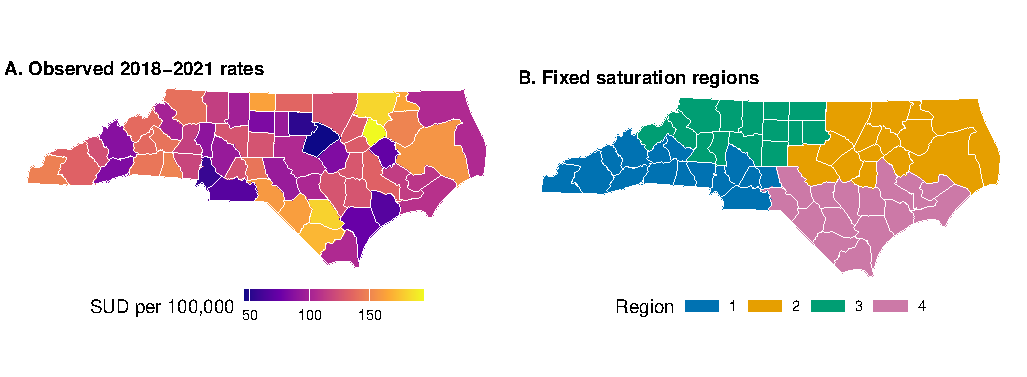
\includegraphics[width=\linewidth]{../figures/compact/nc_planning_map.pdf}
\caption{Observed North Carolina sudden unexpected death (SUD) incidence. (A) SUD rates per 100,000 population aged 18--64 for the 58 service-area clusters, pooled over 2018--2021 (deaths divided by person-years). (B) The fixed four-region partition used by Incidence-Guided Saturation in every year. (C) Annual rates on the same color scale. Each year is analyzed separately, so the year-to-year shifts in panel C explain why some designs' results vary by year (Figure~\ref{fig:nc-mse}). Incidence guides treatment allocation only and does not enter the education outcome.}\label{fig:nc-map}
\end{figure*}
}

\newcommand{\CTJGridFigure}{%
\begin{figure*}[tp]
\centering
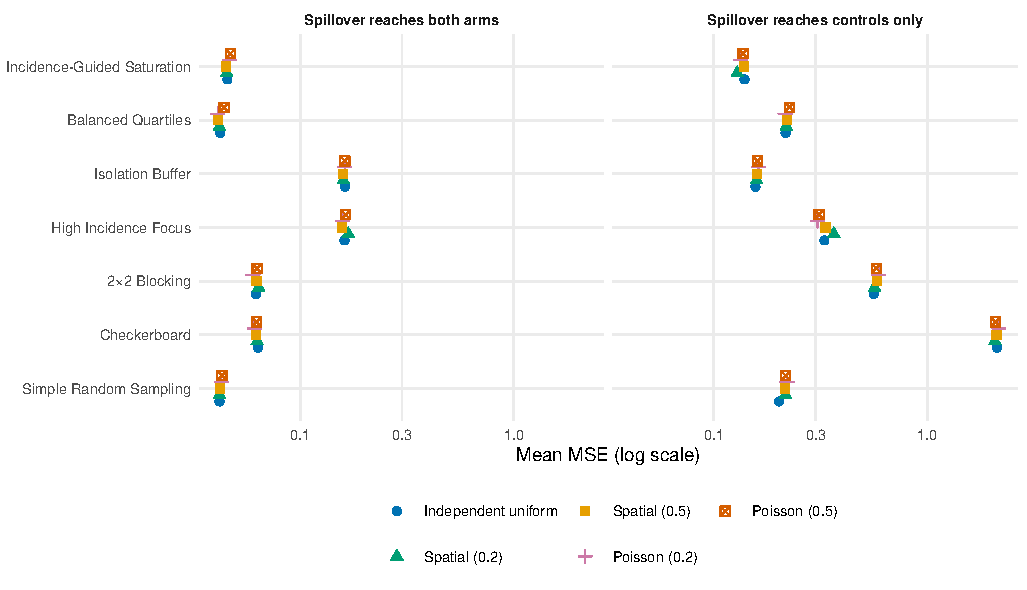
\includegraphics[width=\linewidth]{../figures/compact/grid_accuracy_srs.pdf}
\caption{Grid mean MSE at $\tau=1$ with queen contiguity for the six designs and simple random sampling. Results are shown separately for the five incidence configurations, each averaging the 16 outcome-dependence and spillover-magnitude settings within its spillover regime. Parentheses in the legend give the incidence dependence $\rho_X$. Incidence configuration changes mean MSE little for every design except High Incidence Focus. Horizontal lines are 95\% Monte Carlo intervals over the ten simulated incidence surfaces and are often narrower than the symbols. Designs share surfaces and outcome noise, so Table~\ref{tab:grid-srs} gives the paired comparison of each design with simple random sampling.}\label{fig:grid}
\end{figure*}
}

\newcommand{\CTJAllocationFigure}{%
\begin{figure*}[tp]
\centering
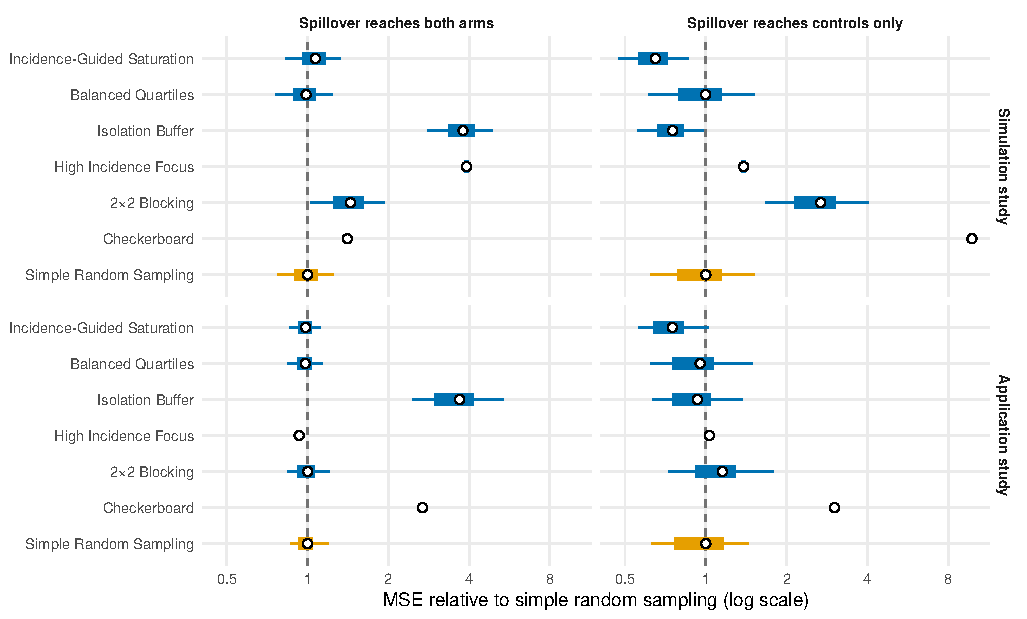
\includegraphics[width=\linewidth]{../figures/compact/allocation_distribution_by_design.pdf}
\caption{Distribution of assignment-specific MSE for the six designs and simple random sampling (SRS), relative to the mean MSE of SRS in the same setting (queen contiguity, $\tau=1$). Figure~\ref{fig:grid} and Table~\ref{tab:grid-srs} report average MSE, whereas this figure shows how MSE varies from one assignment to another (allocation risk). Grid results use all 50 configuration-by-surface units at $\rho\in\{0,0.5\}$ and $\gamma\in\{0.5,0.8\}$, and application results use $\rho\in\{0,0.5\}$ and $\gamma=0.8$ in each year 2018--2021. In the application, $2\times2$ Blocking denotes its spatial-blocking adaptation. Thin lines span the 5th to 95th percentiles of assignments, thick bars the 25th to 75th, and circles mark the mean ratio. Percentiles and means are computed within each setting and then averaged across settings. Outcome noise from the finite number of outcomes per assignment widens the bars, and worst-decile means are reported in the text. A design with one possible assignment per setting appears as a circle only.}\label{fig:alloc-dist}
\end{figure*}
}

\newcommand{\CTJMeanFigure}{%
\begin{figure*}[tp]
\centering
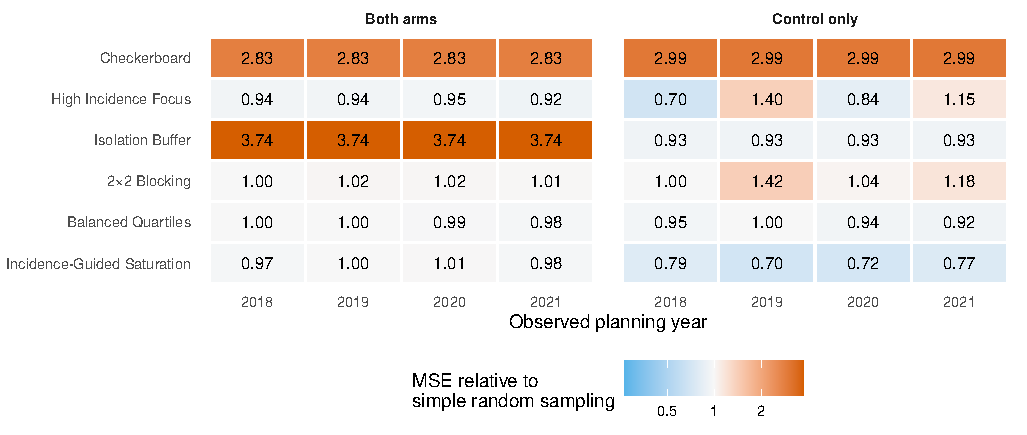
\includegraphics[width=\linewidth]{../figures/compact/nc_annual_accuracy_six.pdf}
\caption{Application mean MSE by year, divided by the mean MSE of simple random sampling (SRS) in the same year and spillover regime, for the six designs with queen contiguity. Each cell averages six $\rho$ and $\gamma$ settings. Blue indicates lower error than SRS and orange higher error, on a logarithmic color scale. SRS mean MSE is 0.07638 under both arms and 0.30761 under control-only spillover. In the application, $2\times2$ Blocking denotes its spatial-blocking adaptation. Absolute MSE, bias and coverage are in the SI.}\label{fig:nc-mse}
\end{figure*}
}
